% Options for packages loaded elsewhere
\PassOptionsToPackage{unicode}{hyperref}
\PassOptionsToPackage{hyphens}{url}
\PassOptionsToPackage{dvipsnames,svgnames*,x11names*}{xcolor}
%
\documentclass[
  ignorenonframetext,
]{beamer}
\usepackage{pgfpages}
\setbeamertemplate{caption}[numbered]
\setbeamertemplate{caption label separator}{: }
\setbeamercolor{caption name}{fg=normal text.fg}
\beamertemplatenavigationsymbolsempty
% Prevent slide breaks in the middle of a paragraph
\widowpenalties 1 10000
\raggedbottom
\setbeamertemplate{part page}{
  \centering
  \begin{beamercolorbox}[sep=16pt,center]{part title}
    \usebeamerfont{part title}\insertpart\par
  \end{beamercolorbox}
}
\setbeamertemplate{section page}{
  \centering
  \begin{beamercolorbox}[sep=12pt,center]{part title}
    \usebeamerfont{section title}\insertsection\par
  \end{beamercolorbox}
}
\setbeamertemplate{subsection page}{
  \centering
  \begin{beamercolorbox}[sep=8pt,center]{part title}
    \usebeamerfont{subsection title}\insertsubsection\par
  \end{beamercolorbox}
}
\AtBeginPart{
  \frame{\partpage}
}
\AtBeginSection{
  \ifbibliography
  \else
    \frame{\sectionpage}
  \fi
}
\AtBeginSubsection{
  \frame{\subsectionpage}
}
\usepackage{lmodern}
\usepackage{amssymb,amsmath}
\usepackage{ifxetex,ifluatex}
\ifnum 0\ifxetex 1\fi\ifluatex 1\fi=0 % if pdftex
  \usepackage[T1]{fontenc}
  \usepackage[utf8]{inputenc}
  \usepackage{textcomp} % provide euro and other symbols
\else % if luatex or xetex
  \usepackage{unicode-math}
  \defaultfontfeatures{Scale=MatchLowercase}
  \defaultfontfeatures[\rmfamily]{Ligatures=TeX,Scale=1}
\fi
% Use upquote if available, for straight quotes in verbatim environments
\IfFileExists{upquote.sty}{\usepackage{upquote}}{}
\IfFileExists{microtype.sty}{% use microtype if available
  \usepackage[]{microtype}
  \UseMicrotypeSet[protrusion]{basicmath} % disable protrusion for tt fonts
}{}
\makeatletter
\@ifundefined{KOMAClassName}{% if non-KOMA class
  \IfFileExists{parskip.sty}{%
    \usepackage{parskip}
  }{% else
    \setlength{\parindent}{0pt}
    \setlength{\parskip}{6pt plus 2pt minus 1pt}}
}{% if KOMA class
  \KOMAoptions{parskip=half}}
\makeatother
\usepackage{xcolor}
\IfFileExists{xurl.sty}{\usepackage{xurl}}{} % add URL line breaks if available
\IfFileExists{bookmark.sty}{\usepackage{bookmark}}{\usepackage{hyperref}}
\hypersetup{
  pdftitle={Simulation and Randomization},
  pdfauthor={Zack Treisman},
  colorlinks=true,
  linkcolor=Maroon,
  filecolor=Maroon,
  citecolor=blue,
  urlcolor=Blue,
  pdfcreator={LaTeX via pandoc}}
\urlstyle{same} % disable monospaced font for URLs
\newif\ifbibliography
\usepackage{color}
\usepackage{fancyvrb}
\newcommand{\VerbBar}{|}
\newcommand{\VERB}{\Verb[commandchars=\\\{\}]}
\DefineVerbatimEnvironment{Highlighting}{Verbatim}{commandchars=\\\{\}}
% Add ',fontsize=\small' for more characters per line
\usepackage{framed}
\definecolor{shadecolor}{RGB}{248,248,248}
\newenvironment{Shaded}{\begin{snugshade}}{\end{snugshade}}
\newcommand{\AlertTok}[1]{\textcolor[rgb]{0.94,0.16,0.16}{#1}}
\newcommand{\AnnotationTok}[1]{\textcolor[rgb]{0.56,0.35,0.01}{\textbf{\textit{#1}}}}
\newcommand{\AttributeTok}[1]{\textcolor[rgb]{0.77,0.63,0.00}{#1}}
\newcommand{\BaseNTok}[1]{\textcolor[rgb]{0.00,0.00,0.81}{#1}}
\newcommand{\BuiltInTok}[1]{#1}
\newcommand{\CharTok}[1]{\textcolor[rgb]{0.31,0.60,0.02}{#1}}
\newcommand{\CommentTok}[1]{\textcolor[rgb]{0.56,0.35,0.01}{\textit{#1}}}
\newcommand{\CommentVarTok}[1]{\textcolor[rgb]{0.56,0.35,0.01}{\textbf{\textit{#1}}}}
\newcommand{\ConstantTok}[1]{\textcolor[rgb]{0.00,0.00,0.00}{#1}}
\newcommand{\ControlFlowTok}[1]{\textcolor[rgb]{0.13,0.29,0.53}{\textbf{#1}}}
\newcommand{\DataTypeTok}[1]{\textcolor[rgb]{0.13,0.29,0.53}{#1}}
\newcommand{\DecValTok}[1]{\textcolor[rgb]{0.00,0.00,0.81}{#1}}
\newcommand{\DocumentationTok}[1]{\textcolor[rgb]{0.56,0.35,0.01}{\textbf{\textit{#1}}}}
\newcommand{\ErrorTok}[1]{\textcolor[rgb]{0.64,0.00,0.00}{\textbf{#1}}}
\newcommand{\ExtensionTok}[1]{#1}
\newcommand{\FloatTok}[1]{\textcolor[rgb]{0.00,0.00,0.81}{#1}}
\newcommand{\FunctionTok}[1]{\textcolor[rgb]{0.00,0.00,0.00}{#1}}
\newcommand{\ImportTok}[1]{#1}
\newcommand{\InformationTok}[1]{\textcolor[rgb]{0.56,0.35,0.01}{\textbf{\textit{#1}}}}
\newcommand{\KeywordTok}[1]{\textcolor[rgb]{0.13,0.29,0.53}{\textbf{#1}}}
\newcommand{\NormalTok}[1]{#1}
\newcommand{\OperatorTok}[1]{\textcolor[rgb]{0.81,0.36,0.00}{\textbf{#1}}}
\newcommand{\OtherTok}[1]{\textcolor[rgb]{0.56,0.35,0.01}{#1}}
\newcommand{\PreprocessorTok}[1]{\textcolor[rgb]{0.56,0.35,0.01}{\textit{#1}}}
\newcommand{\RegionMarkerTok}[1]{#1}
\newcommand{\SpecialCharTok}[1]{\textcolor[rgb]{0.00,0.00,0.00}{#1}}
\newcommand{\SpecialStringTok}[1]{\textcolor[rgb]{0.31,0.60,0.02}{#1}}
\newcommand{\StringTok}[1]{\textcolor[rgb]{0.31,0.60,0.02}{#1}}
\newcommand{\VariableTok}[1]{\textcolor[rgb]{0.00,0.00,0.00}{#1}}
\newcommand{\VerbatimStringTok}[1]{\textcolor[rgb]{0.31,0.60,0.02}{#1}}
\newcommand{\WarningTok}[1]{\textcolor[rgb]{0.56,0.35,0.01}{\textbf{\textit{#1}}}}
\usepackage{graphicx,grffile}
\makeatletter
\def\maxwidth{\ifdim\Gin@nat@width>\linewidth\linewidth\else\Gin@nat@width\fi}
\def\maxheight{\ifdim\Gin@nat@height>\textheight\textheight\else\Gin@nat@height\fi}
\makeatother
% Scale images if necessary, so that they will not overflow the page
% margins by default, and it is still possible to overwrite the defaults
% using explicit options in \includegraphics[width, height, ...]{}
\setkeys{Gin}{width=\maxwidth,height=\maxheight,keepaspectratio}
% Set default figure placement to htbp
\makeatletter
\def\fps@figure{htbp}
\makeatother
\setlength{\emergencystretch}{3em} % prevent overfull lines
\providecommand{\tightlist}{%
  \setlength{\itemsep}{0pt}\setlength{\parskip}{0pt}}
\setcounter{secnumdepth}{-\maxdimen} % remove section numbering

\pgfdeclareimage[width=3.5cm]{mcslogo}{../western_logo_hor_MCS_3C_pos.pdf}
\pgfdeclareimage[width=1cm]{ccbysa}{../ccbysa88x31.png}
\titlegraphic{\href{http://creativecommons.org/licenses/by-sa/4.0/}{\pgfuseimage{ccbysa}}
\hfill
\href{https://western.edu/program/mathematics/}{\pgfuseimage{mcslogo}}}
%\usecolortheme{wcu}
%\institute{Western Colorado University}
%\setbeamertemplate{navigation symbols}{}

\title{Simulation and Randomization}
\author{Zack Treisman}
\date{Spring 2021}

\begin{document}
\frame{\titlepage}

\begin{frame}[fragile]{Philosophy}
\protect\hypertarget{philosophy}{}

Now that we have the components for building models, we need to study
how to evaluate and use our models.

One of the things that having a model (and a computer) allows us to do
is generate simulated data. With simulated data we can:

\begin{itemize}
\tightlist
\item
  Compare models to data (hypothesis testing)
\item
  Make predictions (confidence intervals)
\item
  Plan data collection (power analysis)
\end{itemize}

Since we'll be generating random numbers in these slides, I'll set a
seed now to initialize the process.

\begin{Shaded}
\begin{Highlighting}[]
\KeywordTok{set.seed}\NormalTok{(}\DecValTok{222}\NormalTok{)}
\end{Highlighting}
\end{Shaded}

\end{frame}

\begin{frame}[fragile]{A one variable example}
\protect\hypertarget{a-one-variable-example}{}

A study in Kenward et al. (2004) examined sexual dimorphism in New
Caledonian crows. Sex and weight for 18 birds were recorded.

\begin{Shaded}
\begin{Highlighting}[]
\KeywordTok{ggplot}\NormalTok{(crows, }\KeywordTok{aes}\NormalTok{(weight, sex))}\OperatorTok{+}\KeywordTok{geom_point}\NormalTok{()}
\end{Highlighting}
\end{Shaded}

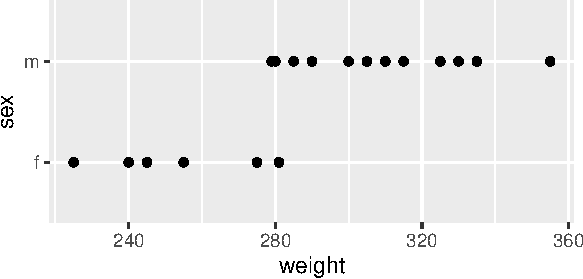
\includegraphics{simulation_files/figure-beamer/unnamed-chunk-4-1.pdf}

\end{frame}

\begin{frame}[fragile]{Crow example (cont.)}
\protect\hypertarget{crow-example-cont.}{}

This is a classic scenario that calls for a \(t\)-test.

\begin{Shaded}
\begin{Highlighting}[]
\KeywordTok{t.test}\NormalTok{(weight}\OperatorTok{~}\NormalTok{sex, }\DataTypeTok{data =}\NormalTok{ crows)}
\end{Highlighting}
\end{Shaded}

\begin{verbatim}
## 
##  Welch Two Sample t-test
## 
## data:  weight by sex
## t = -4.9918, df = 11.221, p-value = 0.000384
## alternative hypothesis: true difference in means is not equal to 0
## 95 percent confidence interval:
##  -80.03218 -31.13449
## sample estimates:
## mean in group f mean in group m 
##        253.5000        309.0833
\end{verbatim}

\end{frame}

\begin{frame}[fragile]{Crow example (cont. 2)}
\protect\hypertarget{crow-example-cont.-2}{}

Alternatively, we could model the null hypothesis of no difference by
\textbf{randomizing} the data. What would these data look like if we had
the same eighteen weights but randomly reassigned to the birds?

\scriptsize

\begin{Shaded}
\begin{Highlighting}[]
\NormalTok{crows}\OperatorTok{$}\NormalTok{shuffled_weight <-}\StringTok{ }\KeywordTok{sample}\NormalTok{(crows}\OperatorTok{$}\NormalTok{weight, }\KeywordTok{length}\NormalTok{(crows}\OperatorTok{$}\NormalTok{weight))}
\KeywordTok{ggplot}\NormalTok{(crows, }\KeywordTok{aes}\NormalTok{(shuffled_weight, sex))}\OperatorTok{+}\KeywordTok{geom_point}\NormalTok{()}
\end{Highlighting}
\end{Shaded}

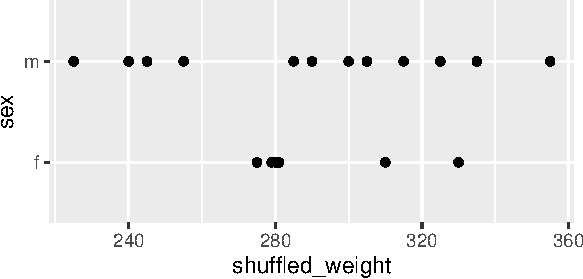
\includegraphics{simulation_files/figure-beamer/unnamed-chunk-6-1.pdf}

\end{frame}

\begin{frame}[fragile]{Crow example (cont 3.)}
\protect\hypertarget{crow-example-cont-3.}{}

Repeat the shuffle many times, and see how our data compare. We'll use
the same statistic that the \(t\)-test used: difference in means between
groups.

\scriptsize

\begin{Shaded}
\begin{Highlighting}[]
\NormalTok{obs <-}\StringTok{ }\KeywordTok{mean}\NormalTok{(crows}\OperatorTok{$}\NormalTok{weight[crows}\OperatorTok{$}\NormalTok{sex}\OperatorTok{==}\StringTok{"f"}\NormalTok{])}\OperatorTok{-}
\StringTok{       }\KeywordTok{mean}\NormalTok{(crows}\OperatorTok{$}\NormalTok{weight[crows}\OperatorTok{$}\NormalTok{sex}\OperatorTok{==}\StringTok{"m"}\NormalTok{])}
\NormalTok{num_sim <-}\StringTok{ }\DecValTok{10000}
\NormalTok{diffs <-}\StringTok{ }\KeywordTok{numeric}\NormalTok{(num_sim)}
\ControlFlowTok{for}\NormalTok{(i }\ControlFlowTok{in} \DecValTok{1}\OperatorTok{:}\NormalTok{num_sim)\{}
\NormalTok{  sim_weight <-}\StringTok{ }\KeywordTok{sample}\NormalTok{(crows}\OperatorTok{$}\NormalTok{weight, }\KeywordTok{length}\NormalTok{(crows}\OperatorTok{$}\NormalTok{weight))}
\NormalTok{  diffs[i] <-}\StringTok{ }\KeywordTok{mean}\NormalTok{(sim_weight[crows}\OperatorTok{$}\NormalTok{sex}\OperatorTok{==}\StringTok{"f"}\NormalTok{])}\OperatorTok{-}
\StringTok{              }\KeywordTok{mean}\NormalTok{(sim_weight[crows}\OperatorTok{$}\NormalTok{sex}\OperatorTok{==}\StringTok{"m"}\NormalTok{])}
\NormalTok{\}}
\KeywordTok{mean}\NormalTok{(}\KeywordTok{abs}\NormalTok{(obs)}\OperatorTok{<=}\KeywordTok{abs}\NormalTok{(diffs)) }
\end{Highlighting}
\end{Shaded}

\begin{verbatim}
## [1] 3e-04
\end{verbatim}

\normalsize

We see three examples in 10,000 runs where the observed difference in
means is at least as large as the observed difference in absolute value.
Note that this matches very closely to the p value of 0.000384 from the
\(t\)-test.

\end{frame}

\begin{frame}[fragile]{Simulating crow weights}
\protect\hypertarget{simulating-crow-weights}{}

Randomization allowed us to test our data against the null theory of
complete independence of the sex and weight variables.

Suppose instead that previous observations lead us to predict that New
Caledonian crows will exhibit sexual dimorphism for weight, with female
weights distributed as \(N(250,20^2)\) and male weights distributed as
\(N(320, 35^2)\).

We will \textbf{simulate} data based on this model.

\scriptsize

\begin{Shaded}
\begin{Highlighting}[]
\NormalTok{diffs <-}\StringTok{ }\KeywordTok{numeric}\NormalTok{(num_sim)}
\ControlFlowTok{for}\NormalTok{(i }\ControlFlowTok{in} \DecValTok{1}\OperatorTok{:}\NormalTok{num_sim)\{}
\NormalTok{  sim <-}\StringTok{ }\KeywordTok{data.frame}\NormalTok{(}\DataTypeTok{sex =} \KeywordTok{c}\NormalTok{(}\KeywordTok{rep}\NormalTok{(}\StringTok{"f"}\NormalTok{, }\DecValTok{6}\NormalTok{), }\KeywordTok{rep}\NormalTok{(}\StringTok{"m"}\NormalTok{, }\DecValTok{12}\NormalTok{)),}
                    \DataTypeTok{weight =} \KeywordTok{c}\NormalTok{(}\KeywordTok{rnorm}\NormalTok{(}\DecValTok{6}\NormalTok{,}\DecValTok{250}\NormalTok{,}\DecValTok{20}\NormalTok{), }\KeywordTok{rnorm}\NormalTok{(}\DecValTok{12}\NormalTok{, }\DecValTok{320}\NormalTok{,}\DecValTok{35}\NormalTok{)))}
\NormalTok{  diffs[i] <-}\StringTok{ }\KeywordTok{mean}\NormalTok{(sim[sim}\OperatorTok{$}\NormalTok{sex}\OperatorTok{==}\StringTok{"f"}\NormalTok{,]}\OperatorTok{$}\NormalTok{weight)}\OperatorTok{-}
\StringTok{              }\KeywordTok{mean}\NormalTok{(sim[sim}\OperatorTok{$}\NormalTok{sex}\OperatorTok{==}\StringTok{"m"}\NormalTok{,]}\OperatorTok{$}\NormalTok{weight)}
\NormalTok{\}}
\KeywordTok{mean}\NormalTok{(}\KeywordTok{abs}\NormalTok{(obs)}\OperatorTok{<=}\KeywordTok{abs}\NormalTok{(diffs)) }
\end{Highlighting}
\end{Shaded}

\begin{verbatim}
## [1] 0.864
\end{verbatim}

\normalsize

The observed difference in weights is at most the simulated difference
86.4\% of the time, not inconsistent with the model.

\end{frame}

\begin{frame}[fragile]{A simple two variable example}
\protect\hypertarget{a-simple-two-variable-example}{}

Simulation can be used to create data based on arbitrarily complicated
models.

A linear function model with normal errors:

\scriptsize

\begin{Shaded}
\begin{Highlighting}[]
\NormalTok{x <-}\StringTok{ }\DecValTok{1}\OperatorTok{:}\DecValTok{20} \CommentTok{# Define inputs}
\NormalTok{a <-}\StringTok{ }\DecValTok{2}\NormalTok{; b <-}\StringTok{ }\DecValTok{1} \CommentTok{# Set parameters}
\NormalTok{y_det <-}\StringTok{ }\NormalTok{a }\OperatorTok{+}\StringTok{ }\NormalTok{b}\OperatorTok{*}\NormalTok{x }\CommentTok{# Compute signal part of output}
\NormalTok{y <-}\StringTok{ }\KeywordTok{rnorm}\NormalTok{(}\DecValTok{20}\NormalTok{, }\DataTypeTok{mean =}\NormalTok{ y_det, }\DataTypeTok{sd =} \DecValTok{2}\NormalTok{) }\CommentTok{# Create noise around the signal}
\KeywordTok{ggplot}\NormalTok{(}\KeywordTok{data.frame}\NormalTok{(}\DataTypeTok{x=}\NormalTok{x, }\DataTypeTok{y=}\NormalTok{y), }\KeywordTok{aes}\NormalTok{(x,y))}\OperatorTok{+}
\StringTok{  }\KeywordTok{geom_point}\NormalTok{() }\OperatorTok{+}\StringTok{ }\KeywordTok{geom_abline}\NormalTok{(}\DataTypeTok{intercept =}\NormalTok{ a, }\DataTypeTok{slope =}\NormalTok{ b) }
\end{Highlighting}
\end{Shaded}

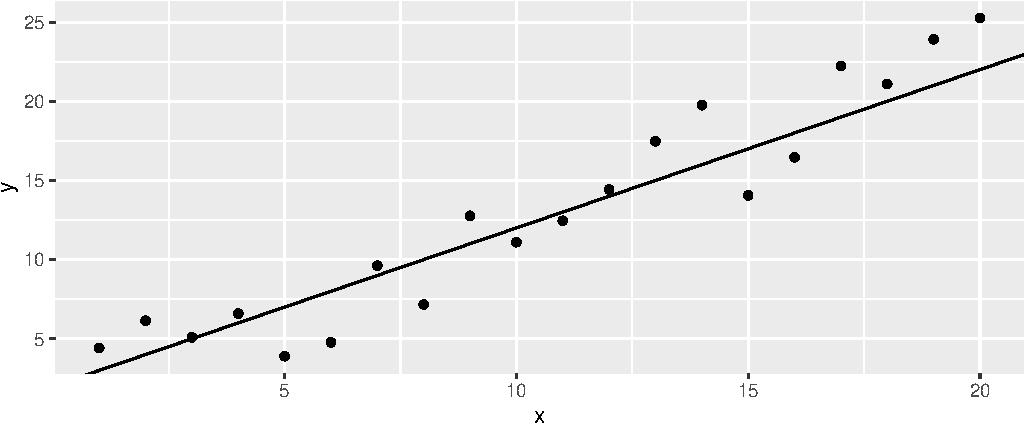
\includegraphics{simulation_files/figure-beamer/unnamed-chunk-9-1.pdf}

\end{frame}

\begin{frame}[fragile]{Another example}
\protect\hypertarget{another-example}{}

A hyperbolic function model with negative binomial errors:

\scriptsize

\begin{Shaded}
\begin{Highlighting}[]
\NormalTok{x <-}\StringTok{ }\KeywordTok{runif}\NormalTok{(}\DecValTok{50}\NormalTok{, }\DataTypeTok{min =} \DecValTok{0}\NormalTok{, }\DataTypeTok{max =} \DecValTok{5}\NormalTok{) }\CommentTok{# Define inputs}
\NormalTok{a <-}\StringTok{ }\DecValTok{20}\NormalTok{; b <-}\StringTok{ }\DecValTok{1}\NormalTok{; k <-}\StringTok{ }\DecValTok{5} \CommentTok{# Set parameters}
\NormalTok{y_det <-}\StringTok{ }\NormalTok{a}\OperatorTok{*}\NormalTok{b}\OperatorTok{/}\NormalTok{(b}\OperatorTok{+}\NormalTok{x) }\CommentTok{# Compute signal part of output}
\NormalTok{y <-}\StringTok{ }\KeywordTok{rnbinom}\NormalTok{(}\DecValTok{50}\NormalTok{, }\DataTypeTok{mu =}\NormalTok{ y_det, }\DataTypeTok{size =}\NormalTok{ k) }\CommentTok{# Create noise}
\KeywordTok{ggplot}\NormalTok{(}\KeywordTok{data.frame}\NormalTok{(}\DataTypeTok{x=}\NormalTok{x, }\DataTypeTok{y=}\NormalTok{y), }\KeywordTok{aes}\NormalTok{(x,y))}\OperatorTok{+}\StringTok{ }
\StringTok{  }\KeywordTok{geom_point}\NormalTok{() }\OperatorTok{+}\StringTok{ }\KeywordTok{geom_function}\NormalTok{(}\DataTypeTok{fun =} \ControlFlowTok{function}\NormalTok{(x) a}\OperatorTok{*}\NormalTok{b}\OperatorTok{/}\NormalTok{(b}\OperatorTok{+}\NormalTok{x) )}
\end{Highlighting}
\end{Shaded}

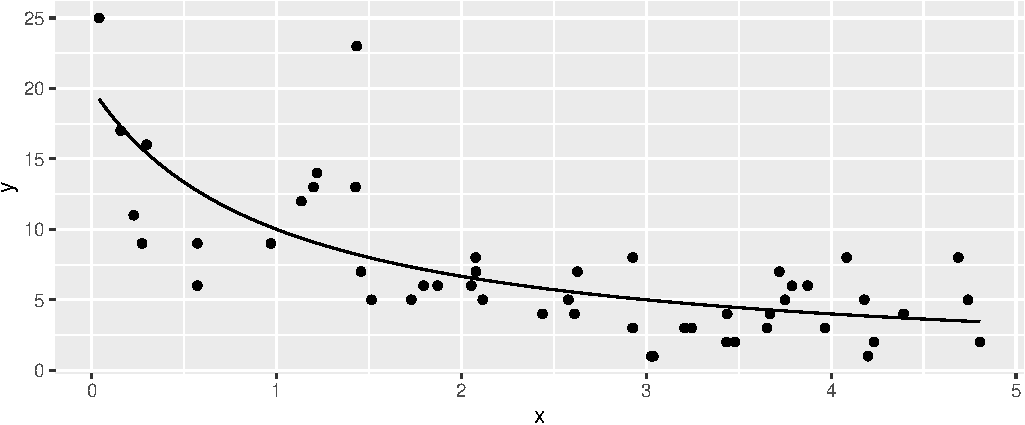
\includegraphics{simulation_files/figure-beamer/unnamed-chunk-10-1.pdf}

\end{frame}

\begin{frame}[fragile]{Adding a categorical predictor}
\protect\hypertarget{adding-a-categorical-predictor}{}

To the previous example, add a grouping factor:

\scriptsize

\begin{Shaded}
\begin{Highlighting}[]
\NormalTok{g <-}\StringTok{ }\KeywordTok{sample}\NormalTok{(}\KeywordTok{c}\NormalTok{(}\DecValTok{0}\NormalTok{,}\DecValTok{1}\NormalTok{), }\DecValTok{50}\NormalTok{, }\DataTypeTok{replace =} \OtherTok{TRUE}\NormalTok{) }\CommentTok{# Define new inputs}
\NormalTok{a <-}\StringTok{ }\DecValTok{20-10}\OperatorTok{*}\NormalTok{g; b <-}\StringTok{ }\DecValTok{1}\OperatorTok{+}\NormalTok{g }\CommentTok{# Redefine parameters to include new input}
\NormalTok{y_det <-}\StringTok{ }\NormalTok{a}\OperatorTok{*}\NormalTok{b}\OperatorTok{/}\NormalTok{(b}\OperatorTok{+}\NormalTok{x) }\CommentTok{# Compute signal part of output}
\NormalTok{y <-}\StringTok{ }\KeywordTok{rnbinom}\NormalTok{(}\DecValTok{50}\NormalTok{, }\DataTypeTok{mu =}\NormalTok{ y_det, }\DataTypeTok{size =}\NormalTok{ k) }\CommentTok{# Create noise}
\KeywordTok{ggplot}\NormalTok{(}\KeywordTok{data.frame}\NormalTok{(}\DataTypeTok{x=}\NormalTok{x,}\DataTypeTok{y=}\NormalTok{y,}\DataTypeTok{g=}\KeywordTok{factor}\NormalTok{(g)), }\KeywordTok{aes}\NormalTok{(x,y, }\DataTypeTok{color=}\NormalTok{g))}\OperatorTok{+}
\StringTok{  }\KeywordTok{geom_point}\NormalTok{() }\OperatorTok{+}\StringTok{ }
\StringTok{  }\KeywordTok{geom_function}\NormalTok{(}\DataTypeTok{fun =} \ControlFlowTok{function}\NormalTok{(x) (}\DecValTok{20}\NormalTok{)}\OperatorTok{/}\NormalTok{(}\DecValTok{1}\OperatorTok{+}\NormalTok{x), }\KeywordTok{aes}\NormalTok{(}\DataTypeTok{color=}\StringTok{"0"}\NormalTok{)) }\OperatorTok{+}
\StringTok{  }\KeywordTok{geom_function}\NormalTok{(}\DataTypeTok{fun =} \ControlFlowTok{function}\NormalTok{(x) (}\DecValTok{10}\NormalTok{)}\OperatorTok{/}\NormalTok{(}\DecValTok{2}\OperatorTok{+}\NormalTok{x), }\KeywordTok{aes}\NormalTok{(}\DataTypeTok{color=}\StringTok{"1"}\NormalTok{))}
\end{Highlighting}
\end{Shaded}

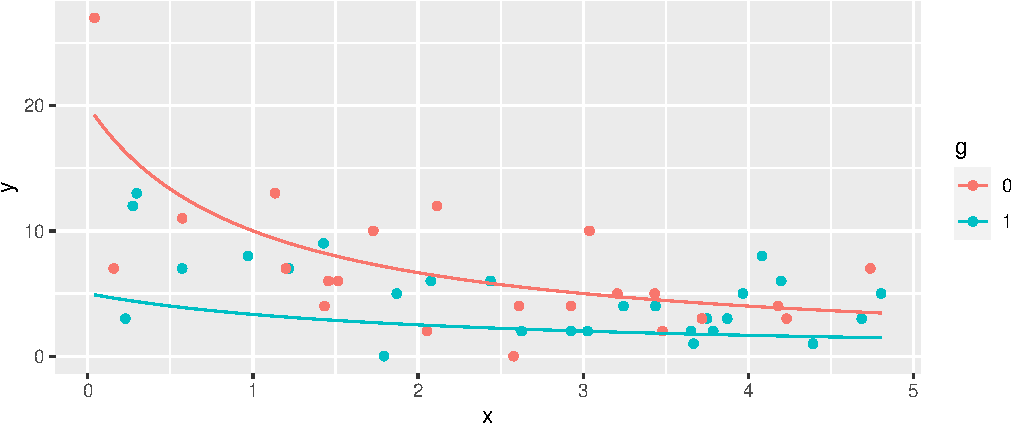
\includegraphics{simulation_files/figure-beamer/unnamed-chunk-11-1.pdf}

\end{frame}

\begin{frame}{A complicated spatial model}
\protect\hypertarget{a-complicated-spatial-model}{}

A study of annual weeds in Pacala and Silander (1990), described in
Section 5.2.2.2 of Bolker (2008) gives an opportunity to see how
complicated models might be built up from simpler components.

The model includes:

\begin{itemize}
\tightlist
\item
  A spatial arrangement of pigweed plants,
\item
  an index of crowding computed from the arrangement,
\item
  an estimate of biomass based on the crowding index, and
\item
  an estimate of seed production based on biomass.
\end{itemize}

We can model each step of this process and chain them together for the
final model.

\end{frame}

\begin{frame}[fragile]{The spatial arrangement}
\protect\hypertarget{the-spatial-arrangement}{}

The spatial arrangement comes from randomly placing parent plants in a
rectangular plot, and then generating offspring plants randomly
dispersed from the parent plants.

First we set parameters for this process: \scriptsize

\begin{Shaded}
\begin{Highlighting}[]
\NormalTok{L =}\StringTok{ }\DecValTok{30} \CommentTok{# consider a 30 by 30 plot }
\NormalTok{nparents =}\StringTok{ }\DecValTok{50} \CommentTok{# and 50 parent plants}
\NormalTok{offspr_per_parent =}\StringTok{ }\DecValTok{10} 
\NormalTok{noffspr =}\StringTok{ }\NormalTok{nparents}\OperatorTok{*}\NormalTok{offspr_per_parent}
\NormalTok{dispdist =}\StringTok{ }\DecValTok{2} \CommentTok{# mean distance from parent to offspring }
\end{Highlighting}
\end{Shaded}

\normalsize

Then we place the parent plants: \scriptsize

\begin{Shaded}
\begin{Highlighting}[]
\NormalTok{parent_x =}\StringTok{ }\KeywordTok{runif}\NormalTok{(nparents,}\DataTypeTok{min=}\DecValTok{0}\NormalTok{,}\DataTypeTok{max=}\NormalTok{L)}
\NormalTok{parent_y =}\StringTok{ }\KeywordTok{runif}\NormalTok{(nparents,}\DataTypeTok{min=}\DecValTok{0}\NormalTok{,}\DataTypeTok{max=}\NormalTok{L)}
\NormalTok{parent_pos <-}\StringTok{ }\KeywordTok{cbind}\NormalTok{(parent_x,parent_y)}
\end{Highlighting}
\end{Shaded}

\normalsize

Then the offspring: \scriptsize

\begin{Shaded}
\begin{Highlighting}[]
\NormalTok{angle =}\StringTok{ }\KeywordTok{runif}\NormalTok{(noffspr,}\DataTypeTok{min=}\DecValTok{0}\NormalTok{,}\DataTypeTok{max=}\DecValTok{2}\OperatorTok{*}\NormalTok{pi) }
\NormalTok{dist =}\StringTok{ }\KeywordTok{rexp}\NormalTok{(noffspr,}\DecValTok{1}\OperatorTok{/}\NormalTok{dispdist)}
\NormalTok{offspr_x =}\StringTok{ }\KeywordTok{rep}\NormalTok{(parent_x,}\DataTypeTok{each=}\NormalTok{offspr_per_parent)}\OperatorTok{+}\KeywordTok{cos}\NormalTok{(angle)}\OperatorTok{*}\NormalTok{dist}
\NormalTok{offspr_y =}\StringTok{ }\KeywordTok{rep}\NormalTok{(parent_y,}\DataTypeTok{each=}\NormalTok{offspr_per_parent)}\OperatorTok{+}\KeywordTok{sin}\NormalTok{(angle)}\OperatorTok{*}\NormalTok{dist}
\NormalTok{pos <-}\StringTok{ }\KeywordTok{cbind}\NormalTok{(offspr_x,offspr_y)}
\end{Highlighting}
\end{Shaded}

\end{frame}

\begin{frame}[fragile]{The spatial arrangement (cont.)}
\protect\hypertarget{the-spatial-arrangement-cont.}{}

Here is a view of the resulting arrangement.

\scriptsize

\begin{Shaded}
\begin{Highlighting}[]
\KeywordTok{ggplot}\NormalTok{()}\OperatorTok{+}
\StringTok{  }\KeywordTok{geom_point}\NormalTok{(}\DataTypeTok{data=}\KeywordTok{as.data.frame}\NormalTok{(pos), }
             \KeywordTok{aes}\NormalTok{(offspr_x, offspr_y, }\DataTypeTok{color=}\StringTok{"child"}\NormalTok{))}\OperatorTok{+}
\StringTok{  }\KeywordTok{geom_point}\NormalTok{(}\DataTypeTok{data=}\KeywordTok{as.data.frame}\NormalTok{(parent_pos), }
             \KeywordTok{aes}\NormalTok{(parent_x, parent_y, }\DataTypeTok{color=}\StringTok{"parent"}\NormalTok{))}\OperatorTok{+}
\StringTok{  }\KeywordTok{labs}\NormalTok{(}\DataTypeTok{x=}\StringTok{""}\NormalTok{, }\DataTypeTok{y=}\StringTok{""}\NormalTok{, }\DataTypeTok{color=}\StringTok{""}\NormalTok{)}
\end{Highlighting}
\end{Shaded}

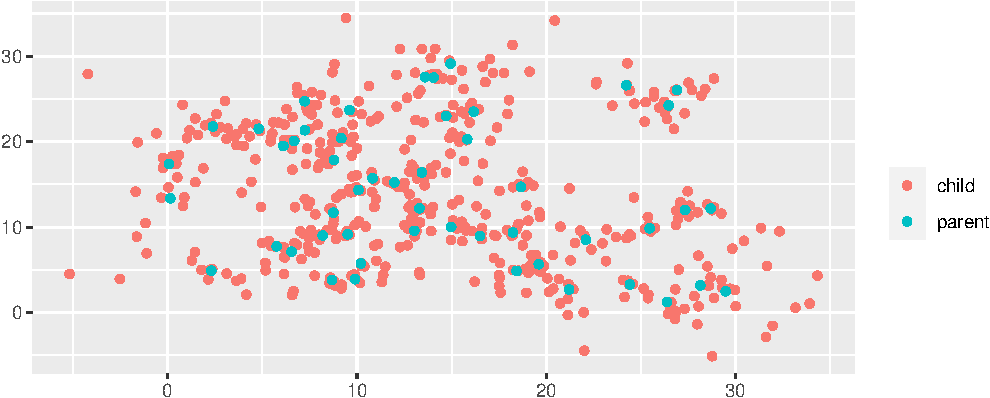
\includegraphics{simulation_files/figure-beamer/unnamed-chunk-15-1.pdf}

\end{frame}

\begin{frame}[fragile]{Computing an index of crowding}
\protect\hypertarget{computing-an-index-of-crowding}{}

For the crowding index, first compute distances between plants.
\scriptsize

\begin{Shaded}
\begin{Highlighting}[]
\NormalTok{ndist <-}\StringTok{ }\KeywordTok{as.matrix}\NormalTok{(}\KeywordTok{dist}\NormalTok{(pos))}
\KeywordTok{heatmap}\NormalTok{(ndist, }\DataTypeTok{Rowv =} \OtherTok{NA}\NormalTok{, }\DataTypeTok{Colv=}\OtherTok{NA}\NormalTok{)}
\end{Highlighting}
\end{Shaded}

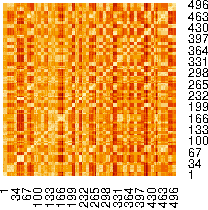
\includegraphics{simulation_files/figure-beamer/unnamed-chunk-16-1.pdf}
\normalsize

Count the number of plants other the plant being considered within a
distance of 2. Multiply the result by 3 and add 1.

\scriptsize

\begin{Shaded}
\begin{Highlighting}[]
\NormalTok{nbrcrowd =}\StringTok{ }\KeywordTok{rowSums}\NormalTok{(ndist}\OperatorTok{<}\DecValTok{2}\NormalTok{)}\OperatorTok{-}\DecValTok{1}
\NormalTok{ci =}\StringTok{ }\NormalTok{nbrcrowd}\OperatorTok{*}\DecValTok{3}
\end{Highlighting}
\end{Shaded}

\end{frame}

\begin{frame}[fragile]{Estimating total biomass}
\protect\hypertarget{estimating-total-biomass}{}

The authors of the study determine a model for total biomass. Their
estimate is based on the competition index and stochastic noise from a
Gamma distribution. \scriptsize

\begin{Shaded}
\begin{Highlighting}[]
\NormalTok{M=}\FloatTok{2.3}\NormalTok{; alpha=}\FloatTok{0.49} \CommentTok{# parameters from Pacala and Silander}
\NormalTok{mass_det=M}\OperatorTok{/}\NormalTok{(}\DecValTok{1}\OperatorTok{+}\NormalTok{ci) }\CommentTok{# deterministic part of the model}
\NormalTok{mass =}\StringTok{ }\KeywordTok{rgamma}\NormalTok{(}\KeywordTok{length}\NormalTok{(mass_det),}\DataTypeTok{scale=}\NormalTok{mass_det,}\DataTypeTok{shape=}\NormalTok{alpha)}
\NormalTok{weeds <-}\StringTok{ }\KeywordTok{data.frame}\NormalTok{(}\DataTypeTok{ci=}\NormalTok{ci, }\DataTypeTok{mass=}\NormalTok{mass, }\DataTypeTok{mass_det=}\NormalTok{mass_det, }
                    \DataTypeTok{x=}\NormalTok{offspr_x, }\DataTypeTok{y=}\NormalTok{offspr_y)}
\KeywordTok{ggplot}\NormalTok{(weeds, }\KeywordTok{aes}\NormalTok{(ci, mass))}\OperatorTok{+}\KeywordTok{geom_point}\NormalTok{()}\OperatorTok{+}\KeywordTok{geom_line}\NormalTok{(}\KeywordTok{aes}\NormalTok{(}\DataTypeTok{y=}\NormalTok{mass_det))}\OperatorTok{+}
\StringTok{  }\KeywordTok{scale_y_log10}\NormalTok{()}\OperatorTok{+}\KeywordTok{labs}\NormalTok{(}\DataTypeTok{x=}\StringTok{"Competition index"}\NormalTok{, }\DataTypeTok{y=}\StringTok{"Biomass"}\NormalTok{)}
\end{Highlighting}
\end{Shaded}

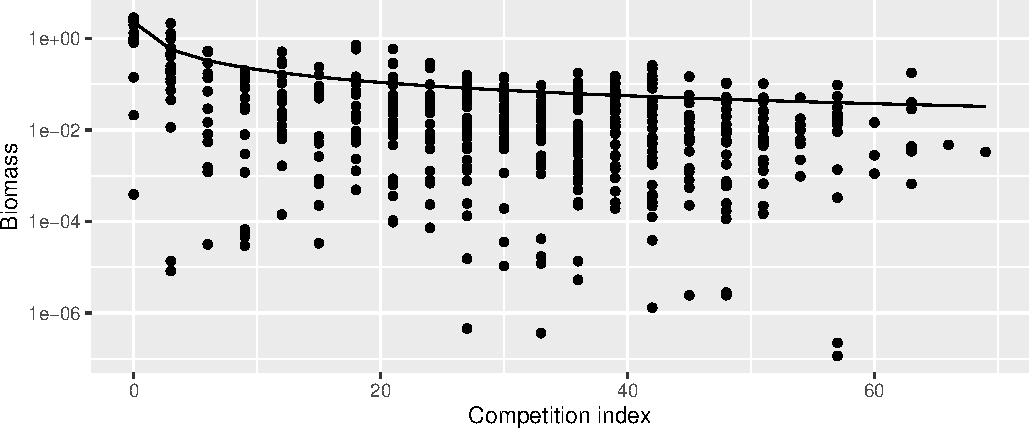
\includegraphics{simulation_files/figure-beamer/unnamed-chunk-18-1.pdf}

\end{frame}

\begin{frame}[fragile]{Estimating seed production}
\protect\hypertarget{estimating-seed-production}{}

Mean seed production is estimated to be proportional to biomass, with
negative binomial noise.

\scriptsize

\begin{Shaded}
\begin{Highlighting}[]
\NormalTok{b =}\StringTok{ }\FloatTok{271.6}\NormalTok{; k =}\StringTok{ }\FloatTok{0.569} \CommentTok{# parameters from Pacala and Silander}
\NormalTok{weeds}\OperatorTok{$}\NormalTok{seed_det <-}\StringTok{ }\NormalTok{b}\OperatorTok{*}\NormalTok{mass }\CommentTok{# the deterministic part of the model}
\NormalTok{weeds}\OperatorTok{$}\NormalTok{seed <-}\StringTok{ }\KeywordTok{rnbinom}\NormalTok{(}\KeywordTok{length}\NormalTok{(weeds}\OperatorTok{$}\NormalTok{seed_det),}\DataTypeTok{mu=}\NormalTok{weeds}\OperatorTok{$}\NormalTok{seed_det,}\DataTypeTok{size=}\NormalTok{k)}
\KeywordTok{ggplot}\NormalTok{(weeds,}\KeywordTok{aes}\NormalTok{(mass,seed}\OperatorTok{+}\DecValTok{1}\NormalTok{))}\OperatorTok{+}\KeywordTok{geom_point}\NormalTok{()}\OperatorTok{+}\KeywordTok{geom_line}\NormalTok{(}\KeywordTok{aes}\NormalTok{(}\DataTypeTok{y=}\NormalTok{seed_det}\OperatorTok{+}\DecValTok{1}\NormalTok{))}\OperatorTok{+}
\StringTok{  }\KeywordTok{geom_line}\NormalTok{(}\KeywordTok{aes}\NormalTok{(}\DataTypeTok{y=}\KeywordTok{qnbinom}\NormalTok{(}\FloatTok{0.025}\NormalTok{,}\DataTypeTok{mu=}\NormalTok{seed_det,}\DataTypeTok{size=}\NormalTok{k)}\OperatorTok{+}\DecValTok{1}\NormalTok{), }\DataTypeTok{linetype=}\DecValTok{2}\NormalTok{)}\OperatorTok{+}
\StringTok{  }\KeywordTok{geom_line}\NormalTok{(}\KeywordTok{aes}\NormalTok{(}\DataTypeTok{y=}\KeywordTok{qnbinom}\NormalTok{(}\FloatTok{0.975}\NormalTok{,}\DataTypeTok{mu=}\NormalTok{seed_det,}\DataTypeTok{size=}\NormalTok{k)}\OperatorTok{+}\DecValTok{1}\NormalTok{), }\DataTypeTok{linetype=}\DecValTok{2}\NormalTok{)}\OperatorTok{+}
\StringTok{  }\KeywordTok{scale_y_log10}\NormalTok{()}\OperatorTok{+}\KeywordTok{scale_x_log10}\NormalTok{()}\OperatorTok{+}
\StringTok{  }\KeywordTok{labs}\NormalTok{(}\DataTypeTok{x=}\StringTok{"Biomass"}\NormalTok{,}\DataTypeTok{y=}\StringTok{"Seed Production + 1"}\NormalTok{)}
\end{Highlighting}
\end{Shaded}

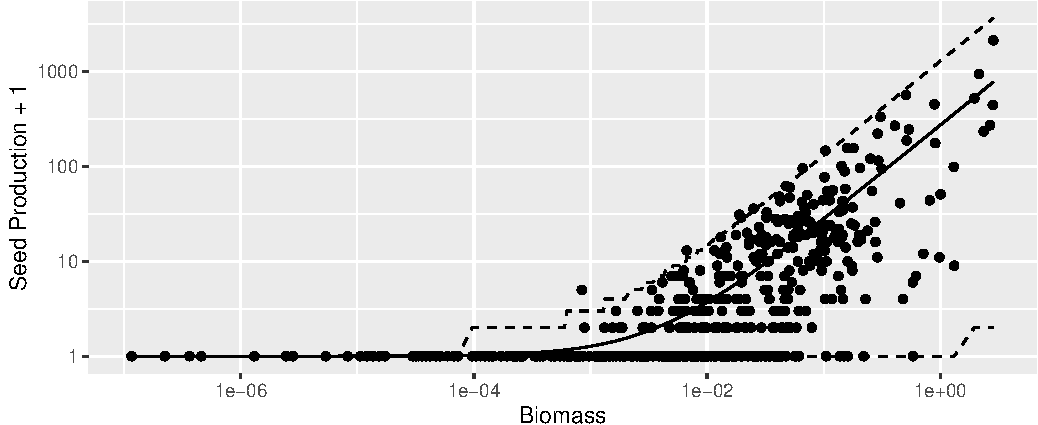
\includegraphics{simulation_files/figure-beamer/unnamed-chunk-19-1.pdf}

\end{frame}

\begin{frame}[fragile]{Simulated distribution of total seed production}
\protect\hypertarget{simulated-distribution-of-total-seed-production}{}

\tiny

\begin{Shaded}
\begin{Highlighting}[]
\NormalTok{num_sim <-}\StringTok{ }\DecValTok{1000}\NormalTok{; total_seeds <-}\StringTok{ }\KeywordTok{numeric}\NormalTok{(num_sim)}
\ControlFlowTok{for}\NormalTok{(i }\ControlFlowTok{in} \DecValTok{1}\OperatorTok{:}\NormalTok{num_sim)\{}
\NormalTok{parent_x =}\StringTok{ }\KeywordTok{runif}\NormalTok{(nparents,}\DataTypeTok{min=}\DecValTok{0}\NormalTok{,}\DataTypeTok{max=}\NormalTok{L); parent_y =}\StringTok{ }\KeywordTok{runif}\NormalTok{(nparents,}\DataTypeTok{min=}\DecValTok{0}\NormalTok{,}\DataTypeTok{max=}\NormalTok{L)}
\NormalTok{angle =}\StringTok{ }\KeywordTok{runif}\NormalTok{(noffspr,}\DataTypeTok{min=}\DecValTok{0}\NormalTok{,}\DataTypeTok{max=}\DecValTok{2}\OperatorTok{*}\NormalTok{pi); dist =}\StringTok{ }\KeywordTok{rexp}\NormalTok{(noffspr,}\DecValTok{1}\OperatorTok{/}\NormalTok{dispdist)}
\NormalTok{offspr_x =}\StringTok{ }\KeywordTok{rep}\NormalTok{(parent_x,}\DataTypeTok{each=}\NormalTok{offspr_per_parent)}\OperatorTok{+}\KeywordTok{cos}\NormalTok{(angle)}\OperatorTok{*}\NormalTok{dist}
\NormalTok{offspr_y =}\StringTok{ }\KeywordTok{rep}\NormalTok{(parent_y,}\DataTypeTok{each=}\NormalTok{offspr_per_parent)}\OperatorTok{+}\KeywordTok{sin}\NormalTok{(angle)}\OperatorTok{*}\NormalTok{dist}
\NormalTok{pos <-}\StringTok{ }\KeywordTok{cbind}\NormalTok{(offspr_x,offspr_y); ndist <-}\StringTok{ }\KeywordTok{as.matrix}\NormalTok{(}\KeywordTok{dist}\NormalTok{(pos))}
\NormalTok{nbrcrowd =}\StringTok{ }\KeywordTok{rowSums}\NormalTok{(ndist}\OperatorTok{<}\DecValTok{2}\NormalTok{)}\OperatorTok{-}\DecValTok{1}\NormalTok{; ci =}\StringTok{ }\NormalTok{nbrcrowd}\OperatorTok{*}\DecValTok{3}\NormalTok{; mass_det=M}\OperatorTok{/}\NormalTok{(}\DecValTok{1}\OperatorTok{+}\NormalTok{ci)}
\NormalTok{mass =}\StringTok{ }\KeywordTok{rgamma}\NormalTok{(}\KeywordTok{length}\NormalTok{(mass_det),}\DataTypeTok{scale=}\NormalTok{mass_det,}\DataTypeTok{shape=}\NormalTok{alpha)}
\NormalTok{seed_det <-}\StringTok{ }\NormalTok{b}\OperatorTok{*}\NormalTok{mass ; seed <-}\StringTok{ }\KeywordTok{rnbinom}\NormalTok{(}\KeywordTok{length}\NormalTok{(seed_det),}\DataTypeTok{mu=}\NormalTok{seed_det,}\DataTypeTok{size=}\NormalTok{k)}
\NormalTok{total_seeds[i] <-}\StringTok{ }\KeywordTok{sum}\NormalTok{(seed)}
\NormalTok{\}}
\KeywordTok{hist}\NormalTok{(total_seeds)}
\end{Highlighting}
\end{Shaded}

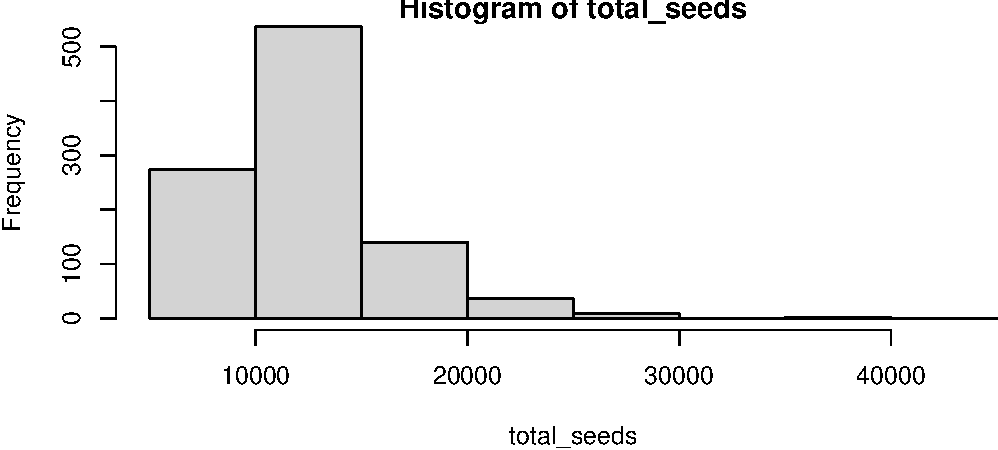
\includegraphics{simulation_files/figure-beamer/unnamed-chunk-20-1.pdf}

\end{frame}

\begin{frame}[fragile]{Hypothesis testing with a simulated distribution}
\protect\hypertarget{hypothesis-testing-with-a-simulated-distribution}{}

We saw in the crow example how to do hypothesis testing with a simulated
distribution:

\begin{itemize}
\tightlist
\item
  Given an observed value of a statistic, calculate the fraction of the
  simulated values that are at least as extreme as the observed value.
  This is the p value.
\end{itemize}

Suppose that in a \(30\times30\) plot with 50 parent plants, each having
10 offspring, you determine that there is a seed set of 23000 seeds.
Test the hypothesis that this seed set is consistent with the model.

\begin{Shaded}
\begin{Highlighting}[]
\KeywordTok{mean}\NormalTok{(total_seeds}\OperatorTok{>=}\DecValTok{23000}\NormalTok{)}
\end{Highlighting}
\end{Shaded}

\begin{verbatim}
## [1] 0.023
\end{verbatim}

At the \(\alpha=0.05\) threshold, this does register as significantly
more seeds than expected. Note this is a one-sided test. In some cases
(crows for example) we can explicitly check a two-sided condition.
Otherwise, doubling p values is a common adjustment to make a one-sided
p value comparable with two-sided ones.

\end{frame}

\begin{frame}[fragile]{Confidence intervals from a simulated
distribution}
\protect\hypertarget{confidence-intervals-from-a-simulated-distribution}{}

Computing confidence intervals from a simulated distribution is
straightforward and can be done using the \texttt{quantile} function.

\begin{Shaded}
\begin{Highlighting}[]
\KeywordTok{quantile}\NormalTok{(total_seeds, }\KeywordTok{c}\NormalTok{(}\FloatTok{0.025}\NormalTok{, }\FloatTok{0.975}\NormalTok{))}
\end{Highlighting}
\end{Shaded}

\begin{verbatim}
##     2.5%    97.5% 
##  7344.65 22333.55
\end{verbatim}

\end{frame}

\begin{frame}{Statistical power}
\protect\hypertarget{statistical-power}{}

In a hypothesis test based on an assumed distribution of a statistic,
there are four important quantities, and and three of them determine the
fourth:

\begin{itemize}
\tightlist
\item
  Sample size (\(n\)) or other model/ experimental parameters
\item
  Effect size (\(\Delta=\mu_a-\mu_0\))
\item
  Significance level (\(\alpha\))
\item
  Power (1-\(\beta\))
\end{itemize}

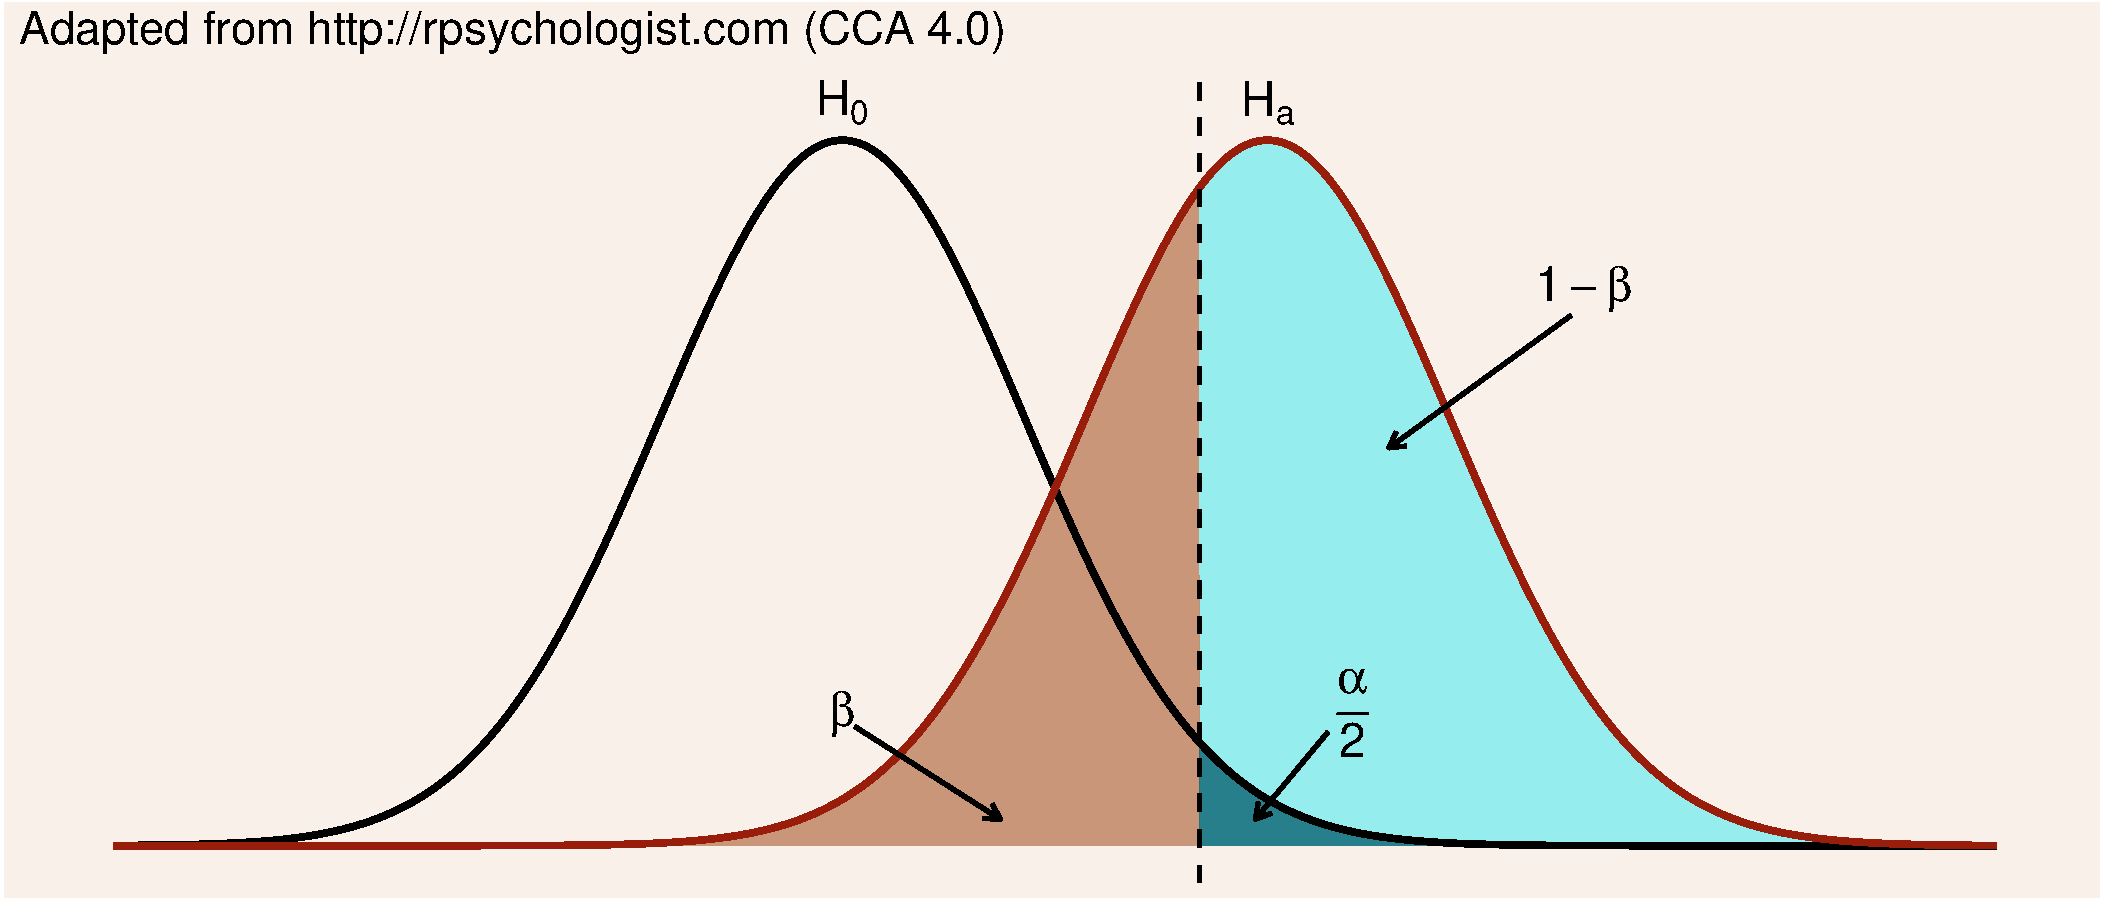
\includegraphics{simulation_files/figure-beamer/unnamed-chunk-23-1.pdf}

\end{frame}

\begin{frame}[fragile]{Power for traditional tests}
\protect\hypertarget{power-for-traditional-tests}{}

Power computers for many standard tests are available in R.

\begin{itemize}
\tightlist
\item
  Suppose male and female crow weights are both approximately normally
  distributed with a pooled standard deviation of 27. How many crows of
  each sex would we need to weigh if we wanted to have a 90\%
  probability of correctly noting a difference in mean weights of 70?
\end{itemize}

\scriptsize

\begin{Shaded}
\begin{Highlighting}[]
\KeywordTok{power.t.test}\NormalTok{(}\DataTypeTok{delta=}\DecValTok{70}\NormalTok{, }\DataTypeTok{sd=}\DecValTok{27}\NormalTok{, }\DataTypeTok{power=}\FloatTok{0.9}\NormalTok{)}
\end{Highlighting}
\end{Shaded}

\begin{verbatim}
## 
##      Two-sample t test power calculation 
## 
##               n = 4.353678
##           delta = 70
##              sd = 27
##       sig.level = 0.05
##           power = 0.9
##     alternative = two.sided
## 
## NOTE: n is number in *each* group
\end{verbatim}

\normalsize

Also see the \texttt{pwr} package.

\end{frame}

\begin{frame}[fragile]{Power computations using simulation}
\protect\hypertarget{power-computations-using-simulation}{}

In a situation where you aren't using a standard statistical test, for
example if you model your data with \texttt{glm} instead of \texttt{lm},
you can use simulation to compute power.

This is what we'll do in the lab.

\end{frame}

\begin{frame}{References}
\protect\hypertarget{references}{}

\hypertarget{refs}{}
\leavevmode\hypertarget{ref-bolker}{}%
Bolker, Benjamin M. 2008. \emph{Ecological Models and Data in R}.
Princeton University Press.

\leavevmode\hypertarget{ref-krwck}{}%
Kenward, Benjamin, Christian Rutz, Alex A. S. Weir, Jackie Chappell, and
Alex Kacelnik. 2004. ``Morphology and Sexual Dimorphism of the New
Caledonian Crow Corvus Moneduloides, with Notes on Its Behaviour and
Ecology.'' \emph{Ibis} 146 (4): 652--60.
\url{https://doi.org/https://doi.org/10.1111/j.1474-919x.2004.00299.x}.

\leavevmode\hypertarget{ref-pacsil}{}%
Pacala, Stephen W., and J. A. Silander. 1990. ``Field Tests of
Neighborhood Population Dynamic Models of Two Annual Weed Species.''
\emph{Ecological Monographs} 60 (1): 113--34.
\url{http://www.jstor.org/stable/1943028}.

\end{frame}

\end{document}
